\documentclass{standalone}
\usepackage{amsfonts,amsmath,tikz,mathtools}

\usetikzlibrary{calc,intersections,arrows}
\usetikzlibrary{shapes.geometric}

\begin{document}

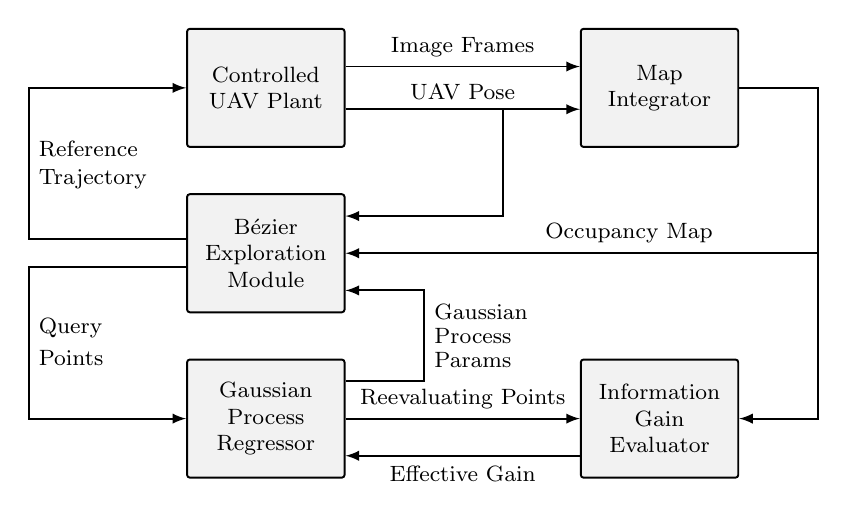
\begin{tikzpicture}[scale=1,>=latex, font=\footnotesize]
\def \sp {0.7pt}
  \tikzstyle{block} = [draw,color=black, fill=black!5, rectangle, rounded corners=1pt,
                       minimum height=1.5cm, minimum width=1.5cm, line width=\sp, text width=2cm,
                       align = center, text=black, inner sep=0]
  \tikzstyle{summer} = [draw,color=black, fill=black!5, circle, text=black,inner sep=2, minimum height=0.8cm]
  \tikzstyle{lines} = [black,line width=\sp,->]
  \tikzstyle{lines2} = [black,line width=\sp,-]
  \tikzstyle{lines3} = [black,line width=\sp,-,dashed]
  \tikzstyle{sum} = [draw,black, fill=black!5, circle, inner sep=1pt, line width=0.7pt]
  \tikzstyle{gain} = [draw, black,line width=0.7pt, fill=black!5,
                      regular polygon, regular polygon sides=3, shape border rotate=90]
  
%%%%%%%%%%%%%%%%%%%%%%%%%%%%%%%%%%%%%%%%%%%%%%%%%%%%%%%%%%%%%%%%%%%%%%%%%%%%%%%

\coordinate (uav_pose) at (0, 0);
\coordinate (map_pose) at (5, 0);
\coordinate (bezier_pose) at (0, -2.1);
\coordinate (gain_pose) at (5, -4.2);
\coordinate (gp_pose) at (0, -4.2);

%%%%%%%%%%%%%%%%%%%%%%%%%%%%%%%%%%%%%%%%%%%%%%%%%%%%%%%%%%%%%%%%%%%%%%%%%%%%%%%

\node[block] (uav) at (uav_pose) {Controlled UAV Plant};
\node[block] (map) at (map_pose) {Map \\ Integrator};
\node[block] (bezier) at (bezier_pose) {Bézier Exploration Module};
\node[block] (gain) at (gain_pose) {Information Gain Evaluator};
\node[block] (gp) at (gp_pose) {Gaussian Process Regressor};

%%%%%%%%%%%%%%%%%%%%%%%%%%%%%%%%%%%%%%%%%%%%%%%%%%%%%%%%%%%%%%%%%%%%%%%%%%%%%%%

\draw[lines] (uav.15) -- node[pos=0.5,above] {Image Frames} (map.165);
\draw[lines] (uav.345) -- node[pos=0.5,above] {UAV Pose} (map.195);
\draw[lines] (uav.345) -- ++ (2,0) |- (bezier.25);
\draw[lines] (map.0) -- ++ (1,0) |- (gain.0);

\draw[lines] (bezier.190) -- ++ (-2,0) |- node[pos=0.3,right] {Points} node[pos=0.2,right] {Query} (gp.180);
\draw[lines] (gp.25) -- ++ (1,0) |- node[pos=0.38,right] {Gaussian} node[pos=0.25,right] {Process} node[pos=0.12,right] {Params} (bezier.335);
\draw[lines] (gp.0) -- node[pos=0.5,above] {Reevaluating Points} (gain.180);
\draw[lines] (gain.205) -- node[pos=0.5,below] {Effective Gain} (gp.335);

\draw[lines] (map.0) -- ++ (1,0) |-  node[pos=0.7,above] {Occupancy Map} (bezier.0);
\draw[lines] (bezier.170) -- ++ (-2,0) |- node[pos=0.3,right] {Reference} node[pos=0.2,right] {Trajectory} (uav.180);

\end{tikzpicture}
\end{document}